\documentclass[]{article}

\usepackage{xcolor}
\usepackage{tikz}
\usepackage{pgfplots}

\newlength{\xdim}

\definecolor{calculate}{HTML}{D7191C}
\definecolor{copyBack}{HTML}{FDAE61}

%opening
\title{Multiprocessor Systems - Assignment I (MPI)}
\author{Adrian Holfter, Lucie Labadie}

\begin{document}

\maketitle

\section{Implementation}

\subsection{MPI-based Blocked Matrix-Matrix Multiplication}

\subsection{MPI-based Laplace Approximation}

\paragraph{} First we chose to write the row-wise MPI-implementation of the Laplace Approximation. So we split the matrix on row dimension only given the number of cores set.
\paragraph{} After splitting the matrix we have to send each part to the workers. Each worker will receive : 
\begin{itemize}
	\item offset : the chunk position in the whole matrix; 
	\item rows : the number of rows the worker have to compute;
	\item  matrix : the matrix part the worker should compute with the extra rows and columns needed for the computation (one after and one before). 
\end{itemize}

\paragraph{} The master will then do its part of the computation and wait to receive the results of the workers. 

\paragraph{} The workers will receive their data and start the computation, after computation they will send back the results to the master : 
\begin{itemize}
	\item offset;
	\item result matrix.
\end{itemize}
We do not need to send the number of rows again since it is already known by the master. 

\paragraph{} The work executed by each worker and the master starts by exchanging the extra rows on top and bottom. During the first turn this operation is not really necessary but it will serve for the next since it is needed for the further computations. The first pass of computation is executed respecting the turn we are in (ODD or EVEN). Now we need to check stopping condition by taking the maximum of each row and keeping only the biggest. To do so we have to synchronized this value between all the workers. Each worker is computing its own maximum value and send it to the master which will check either to stop or not and send the result back the workers. Then we can change the turn (ODD or EVEN) and go back to top of the loop until it is finished. 

%pseudo code ??

\section{Measurements}

\subsection{MPI-based Blocked Matrix-Matrix Multiplication}

The measurements were taken on the \emph{kraken.tek.bth.se} Server. The executables were compiled with the \texttt{-O3} option, to enable compiler optimizations. Every measurement was taken 10 times and the smallest value was used. Table \ref{tab:matrix-mult-runtime} shows the runtimes of the different versions.

\begin{figure}[h]
	\centering
	\begin{tabular}{|l|r|}
		\hline
		\textbf{Version} & \textbf{shortest runtime [s]} \\
		\hline
		Sequential single-threaded & 30.40 \\ 
		\hline 
		MPI 1 thread & 2.54 \\ 
		\hline 
		MPI 2 threads & 0.95 \\ 
		\hline 
		MPI 4 threads & 0.57 \\ 
		\hline 
		MPI 8 threads & 0.47 \\ 
		\hline 
	\end{tabular} 
	\caption{Runtime comparison for matrix multiplication}
	\label{tab:matrix-mult-runtime}
\end{figure}

Figure \ref{fig:maxtrix-mult-chart} shows the runtime breakdown for the MPI version per number of workers. It becomes clear that the percentage of time spent copying back the result matrix increases rapidly, which is because every worker sends back the \emph{whole} \texttt{C} matrix, even though only a small part of it actually contains work results.

\begin{figure}[h]
	\centering
	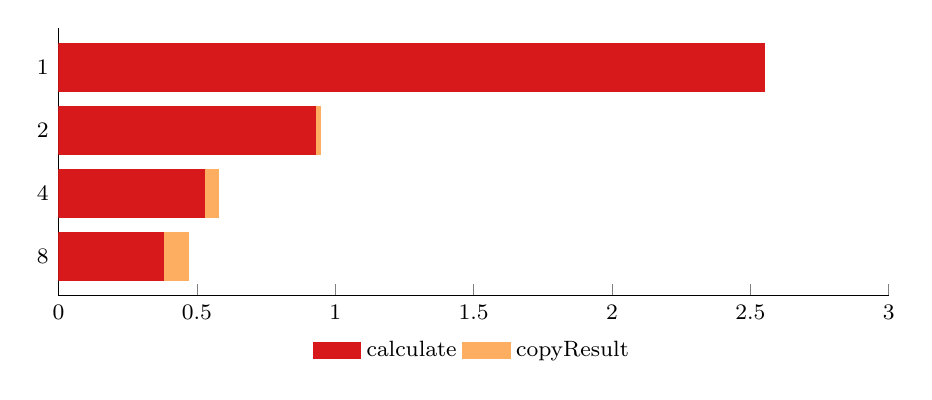
\begin{tikzpicture}
	\begin{axis}[
	xbar stacked,
	legend style={
		legend columns=4,
		at={(xticklabel cs:0.5)},
		anchor=north,
		draw=none
	},
	ytick=data,
	axis y line*=none,
	axis x line*=bottom,
	tick label style={font=\footnotesize},
	legend style={font=\footnotesize},
	label style={font=\footnotesize},
	xtick={0, 0.5, 1.0, 1.5, 2.0, 2.5, 3.0},
	width=1.0\textwidth,
	bar width=6mm,
	xlabel={Time in ms},
	yticklabels={1, 2, 4, 8},
	xmin=0,
	xmax=3.0,
	area legend,
	y=8mm,
	enlarge y limits={abs=0.625},
	]
	\addplot[calculate,fill=calculate] coordinates
	{(2.55,3) (0.927,2) (0.527,1) (0.380,0)};
	\addplot[copyBack,fill=copyBack] coordinates
	{(0.0,3) (0.02,2) (0.05,1) (0.09,0)};
	\legend{calculate, copyResult}
	\end{axis}  
	\end{tikzpicture}
	\caption{Runtime breakdown for matrix multiplication per number of workers}
	\label{fig:maxtrix-mult-chart}
\end{figure}

\subsection{MPI-based LaPlace Approximation}

\end{document}
